\section{Stereo Reconstruction}
Stereo reconstruction is a powerful way to reconstruct depth of scenes by point correspondences between different views of the scene. There are multiple steps to stereo reconstruction:
\begin{enumerate}
    \item Calibration and estimation of the epipolar geometry (correspondences must lie on a line)
    \item Disparity estimation to find the correspondences
    \item Triangulation: Reconstructing the 3D point from 2D correspondences
\end{enumerate}

\subsection{Epipolar Geometry}
The epipolar geometry is independent of the scene structure. It depends only on the internal camera parameters and their \b{relative} pose.\\
The corresponding point in the other camera must lie on the projected projection ray (epipolar line):

\begin{figure}[h!]
    \centering
    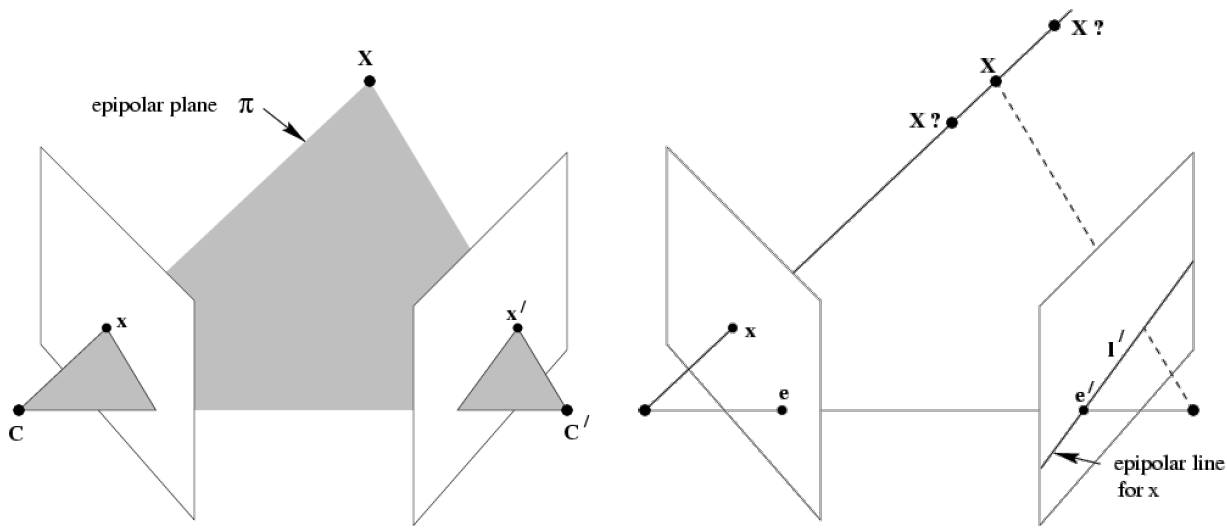
\includegraphics[width=.8\textwidth]{line.png}
\end{figure}

The projection ray itself can be constructed using the camera parameters. The projection of the camera center in the other camera \f{C} is called \b{epipole} \f{\pmb{e}}. All epipolar lines go through the epipole. If it is visible in the image, it is also called \b{focus of expansion}.\\

\b{Fundamental Matrix:\\[0.5em]}
The epipolar geometry is fully described by the so-called fundamental matrix \f{F^{3\times3}} (rank 2). It describes the mapping of an image point in one camera to the corresponding epipolarline in the other camera (homogenous coordinates):
\cf{
    l' = Fx \qquad,\qquad l=F^\top x'\qquad,\qquad x'^\top Fx=0
}
\b{Note:} \f{F} can be estimated from 2D correspondences alone (in contrast to \f{P}).\\

If we know the projection matrices of two cameras, the fundamental matrix can be derived as:
\cf{
    F = [e']_\times P'P^\dagger ,
}
where \f{e'} is the epipole in the second camera with \f{e'=P'C}. \f{C} is obtained by solving \f{PC=0}. \f{P^\dagger} is the pseudo-inverse of \f{P} with \f{P^\dagger :=(P^\top P)^{-1}P^\top}. \f{[e']_\times} denotes the skew-matrix (not included).\\

If we have point correspondences, we can estimate the fundamental matrix without the need of a calibrated camera. Due to the line-constraint from above and the rank-2 constraint, it has 7 degrees of freedom. However, it is easier to over-parametrization with 9 parameters and a constraint on the scale, which leads to the \b{8-point algorithm} (similar to calibration/homography).
\newpage

Here, normalization is even more important, as \f{F} is more sensitive to noise in the correspondences because the pixel positions will be squared (so the error will be squared too).\\
Combining the constraints from \f{N} correspondences we get the linear system \f{Af=0} with \f{A\in\mathbb{R}^{N\times 9}}. The solution is obtained as the singular vector to the smallest singular value of \f{A}.\\ This estimate does usually not satisfy the rank constraint, which can be enforced afterwards by and SVD of \f{F}, setting the smallest singular value to 0.\\

Higher accuracy estimates are obtained by iterative procedures that start with the 8-point algorithm for initialization and then refine the estimate. Iteration is necessary since the distance measures are nonlinear.\\

\b{Reprojection Error:} The F-matrix is estimated together with the reconstructed 3D points. The error between the reprojected 3D points and the 2D points is minimized (bundle adjustment).\\

\b{Outliers:\\[0.5em]}
Estimation methods as introduced can deal with small (Gaussian) errors. However, calculating correspondences can yield a few false matches (e.g. because of occlusion), so called \b{outliers}. These outliers can severely disturb the results, which is why they have to be removed.\\

\b{Random Sample Consensus (RANSAC)} is a method for outlier identification and estimating parameters only from inliers:
\begin{enumerate}
    \item Randomly select subset of mimimum size
    \item Estimate model from this subset
    \item Determine the number of points that are consistent with this model (number of inliers, \b{support})
    \item Repeat these steps with different subsets and choose subset with largest support
    \item Estimate model from all inliers
\end{enumerate}

In practice: You collect 200 point corr. for the image pair. Now you sample 8 random correspondences of the 200, put them into the 8-point-algorithm and get an estimated F-matrix (model). Next you check how good the remaining 192 points fit into the new F-matrix. Choose a treshild and estimate which correspondences are inliers and which are outliers. Repeat the previous steps with different subsets and choose the F-matrix with the most inliers. Then estimate the F-matrix from all these inliers.\\

\b{Note:} The chance of picking a subset consisting only of inlier increases with the number of iterations. It decreases with the size of the subsets (degrees of freedom).\\

\b{Autocalibration:\\[0.5em]}
The F-matrix can be estimated without the need of a calibration tool. This means you can simply take two pictures from different views of an object and perform the calibration with them.\\
The idea: Given the F-matrix we can derive a canonical form of the P-matrices (autocalibration via F-matrix):
\cf{
    P=(I|0)\qquad P'=([e']_\times F|e')\qquad 
}
where \f{e'} is obtained by solving \f{F^\top e'=0}. The first projection matrix (\f{P}) is set as the identity with zero vector to fix the world coordinate system.\\
\b{Problem:} Many other projection matrices satisfy the constraints given by the F-matrix (both P-matrices have a combined total of 22 degrees of freedom, while the F-matrix only has 7). The remaining 15 degrees of freedom describe a 3D projective transformation (which should only have \f{3\times 3}), which leads to \b{projective amiguity}. \f{\to} Metric reconstrucion

\subsection{Metric Reconstruction}
For a metric reconstruction only the internal camera parameters must be known. This fixes 10 of 15 degrees of freedom. We can then derive the relative pose of the two cameras, known as \b{egomotion}, up to a scale factor. Knowing that we can compute the normalized coordinates of the image points as:
\cf{
    \hat{x} = K^{-1}x\qquad,\qquad \hat{x}' = K'^{-1}x'
}
From point correspondences we can estimate the \b{essential matrix} \f{\pmb{E}} with \f{\hat{x}'E\hat{x}=0}. \f{E} is related to \f{F} and the egomotion via:
\cf{
    E=K'^\top FK = [t]_\times R = R[R^\top t]_\times
}
The essential matrix only has 5 d.o.f, while the F-matrix has 7. This means that one can derive \f{E} directly (when knowing the camera parameters). However, \f{E} can also be estimated with the 8-point algorithm enforcing the constraints of rank 2 and the first two singular values being one.\\
Because \f{E} is related to the egomotion, we want to calculate the positions of camera in the images. For that we can decompose \f{E} via SVD into \f{E=U\text{diag}(1,1,0)V^\top} and fix \f{P=(I|0)} for the first image. Due to sign ambiguity of SVD this results in for possible positions (rotations and translations) of the camera in image two, of which only one solution can be true (verification: a single point must be in front of both cameras).\\

Even though metric reconstruction removes the projective ambiguity of autocalibration, there are still some similarity ambiguities left (translation, rotation, scaling). For example: Is an object big and far away or close and small? These ambiguities can partly be answered by landmarks and objects of known size in the scene. The scale amiguity can also be avoided through fixed stereo cameras.

\subsection{Triangulation}
With given correspondences and P-matrices we can traingulate the 3D points. For perfect measurements the following restraints hold:
\cf{
    x=PX\qquad,\qquad x'P'X
}
However, often the image points do not satisfy the epipolar constraint exactly (projection rays miss each other). The solution can be found in the least squares sense.\\

The direction of the projected 3D points must coincide with the image points:
\cf{
    x\times (PX) = 0\qquad,\qquad x'\times (P'X) = 0
}
This results in three constraints for each of the two points, of which two are linearly independent. By combining the restraints we get the linear system \f{AX=0} with \f{A\in\mathbb{R}^{4\times1}}.\\
For projective reconstruction the constraint \f{||X||=1} is added. For metric reconstruction the \f{4^{\text{th}}} \f{X}-component is fixed: \f{X=(X,Y,Z,1)^\top}.\\

\b{Uncertainty in the estimate:\\[0.5em]}
The uncertainty in the exact position of the corresponding point in the other image propagates to the depth estimate. The propagation is more severe the more parallel two rays are.\\
Hence, a large baseline is positive for accurate depth measurements, but it also makes finding corresponding points harder (larger search range, more distortion, more occlusions).
\newpage